\documentclass[11pt]{article}

%============引用宏包 和 自定义命令========================%
\usepackage{CJK}
\usepackage{graphicx}
\usepackage{latexsym,bm}
\usepackage{amsmath}
\usepackage{xcolor}
\usepackage{fancyhdr}
\usepackage{tikz}
\usepackage{slashbox}
\usepackage{colortbl}
\pagestyle{fancy}

%============ 重定义字体、字号命令 =======================%
\newcommand{\hei}{\CJKfamily{hei}}

\begin{document}
\begin{CJK}{UTF8}{gbsn}
%------------------------文章标题---------------------------------------------------------
\rhead{\tt L.J.SHOU 
\includegraphics[scale=0.2]{ICT.eps}}  %页眉
\title{ \textbf{Assignment 2 of Algorithm Design and Analysis}}
\author{L.J.SHOU  寿林钧\\{\slshape No}. \bf 201228013229133}
\date{Oct.22 2012}
\maketitle % 生成题头
%------------------------正文------------------------------------------------------------%
\section{Divide and Conquer(2)}
{\em \sf QUESTION:}\\[1mm]
Try to find the median number from two databases, whose sizes are n respectively in O(lgn) time complexity. \\
{\footnotesize Notes: the given databases can only be accessed through quiries.}\\[1mm]
{\em \sf Pseudo-Code:}\\[1mm]
{\bf {\bf Get-Median}}$(A,B,n,a,b) A, B$ denotes databases;\\
 1: $k=[n/2];$                                 \\
 2: {\bf if} $n=1$ {\bf then}                             \\ 
 3:          {\bf return} min$(A(a+k),B(b+k))$;\\
 4: {\bf endif}\\
 5: {\bf if} $A(a+k)<B(b+k)$ {\bf then}\\
 6:          {\bf return} {\bf Get-Median}$(A,B,k,a+k,b)$;\\
 7: {\bf else}\\
 8:          {\bf return} {\bf Get-Median}$(A,B,k,a,b+k)$;\\
 9: {\bf {\bf endif}}\\
 \\
{\em \sf Complexity Analysis:}\\[1mm]
$T(n)<=T(n/2)+2$\\
As a result, we have $T(n)=O(lgn)$\\

\newpage \section{Sorting(2)}

%\begin{tikzpicture}[thick,smooth,domain=0:4,scale=0.9]
	%\draw[very thin, gray](0,0) grid(12, 4);
	%\draw plot[mark=*] coordinates{(100000,0.04) (1000000,0.4) (10000000,5)}; 
%/end{tikzpicture}
%\begin{pgftranslate}{\pgfpoint{0cm}{1cm}}
%\pgfline{\pgforigin}{\pgfxy(1,0)}
%\end{pgftranslate}

My test results are shown in the followig table, which are based on three random integer arrays whose sizes are 100,000, 1,000,000, 10,000,000 respectively.\par
\centering{\bf \large Comparision of different Sorting Methods}\\[5mm]
%-------------表格1-------------------------------------
\begin{tabular}{|c|c|c|c|}\hline
\backslashbox[2.5cm]{\bf METHODS}{\bf \cellcolor[gray]{.7}  No.}   & $10^5$  & $10^6$ & $10^7$ \\\hline
{\emph MergeSort} & 0.05s    & 0.62s   & 7.07s  \\\hline
\rowcolor[gray]{.7}{\emph QuickSort} & 0.03s    & 0.40s   & 4.75s  \\\hline
{\emph M\_QuickSort} & 0.04s    & 0.42s   & 5.04s  \\\hline
\rowcolor[gray]{.7}{\emph MergeSort\_Stack} & 0.06s    & 0.68s   & 7.71s  \\\hline
{\emph QuickSort\_Stack} & 0.04s    & 0.50s   & 5.72s  \\\hline
\rowcolor[gray]{.7}{\emph M\_QuickSort\_Stack} & 0.04s    & 0.48s   & 5.47s  \\\hline
\end{tabular}\\[5mm]
while if the input integer arrays are already in order, running time VARIES distinctively.\par
%-----------表格2---------------------------------------
\begin{tabular}{|c|c|}\hline
\backslashbox{\bf METHODS.}{\bf \cellcolor[gray]{.7}No.}& $10^5$ \\\hline
 {\emph MergeSort} & 0.04s\\\hline  
\rowcolor[gray]{.7}{\emph QuickSort} & 59.71s\\\hline 
{\emph M\_QuickSort} & 0.02s\\\hline
\rowcolor[gray]{.7}{\emph MergeSort\_Stack} & 0.04s\\\hline
{\emph QuickSort\_Stack} & 59.71s\\\hline
\rowcolor[gray]{.7}{\emph M\_QuickSort\_Stack} & 0.03s\\\hline
\end{tabular}\\[5mm]

%-------------------------插入两张并排的图片----------------------------------------------------
\begin{figure}[!ht]   % !h用来使图片放在段落之间,而非有latex自动放置
\begin{minipage}[b]{0.5\linewidth}
   \centering
   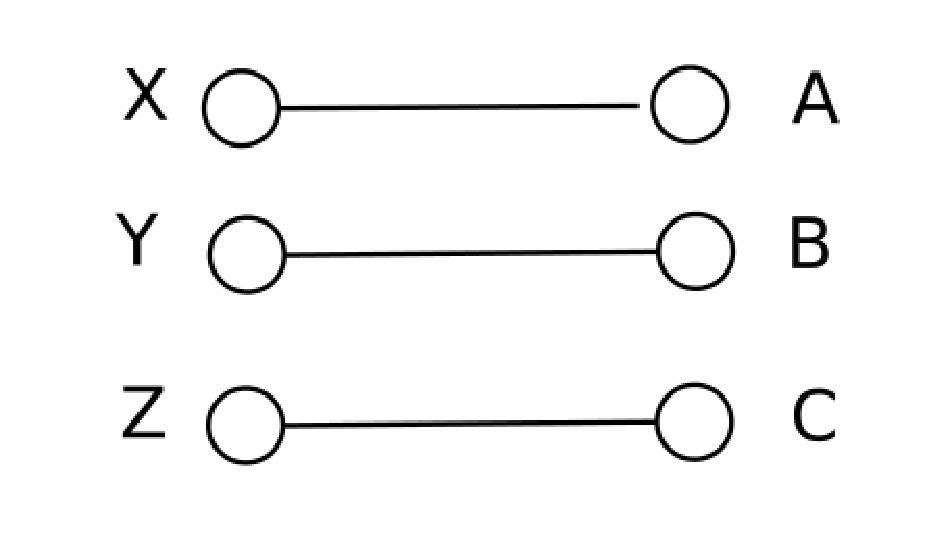
\includegraphics[width=8cm]{stable-matching1.eps}
   \caption{Stable Matching 1}
\end{minipage}
\begin{minipage}[b]{0.5\linewidth}
   \centering
   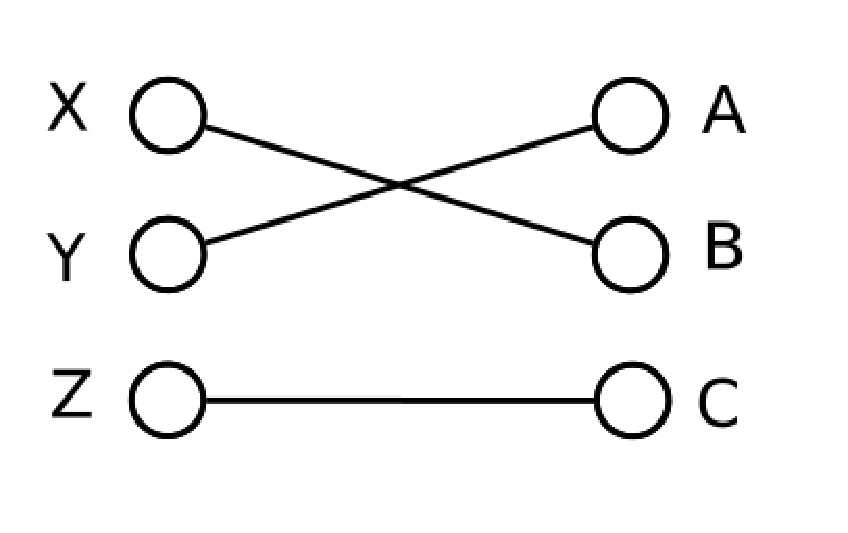
\includegraphics[width=7.5cm]{stable-matching2.eps}
   \caption{Stable Matching 2}
\end{minipage}
\end{figure}

\newpage \end{CJK}
\end{document}
